\subsection{The 404-pair subset and the linear command readout}
\label{sec:current-basis-readout}

On the 404 pairs of main Fig.~\ref*{M-fig:token-structure}, the position-centered shared directions retain $36.5$--$83.6\%$ of the response energy around the fitting-data mean, against $0.5$--$10.2\%$ for clean-feature and $1.3$--$1.9\%$ for random directions: the C1 numbers of the main paper. An exploratory linear readout of the same 16 coordinates predicts the change in the first five commands better than predicting no change at L18 in all four families, but not at L1 and L9 (Table~\ref{tab:current-basis-control}; main Fig.~\ref*{M-fig:token-structure}b). This supports main Sec.~\ref*{M-sec:shared} with two qualifications: at L18 the shared coordinates predict no better than clean-feature coordinates, and first flow predicts better than any set of coordinates.

\paragraph{What the readout is compared with.}
Affine readouts are compared on the same held-out cases with predicting no change (absolute accuracy), clean-feature and random coordinates (choice of directions), the full hidden response (prediction before compression) and first flow (information beyond a downstream output; it beats no change in every family). Table~\ref{tab:current-basis-control} puts all layers on one translation-error scale; the figures keep all command components.

\paragraph{Retention and prediction peak at different layers on the same cases.}
At L1 and L9, shared-direction coordinates reduce affine translation error by $20$--$75\%$ and $27$--$71\%$ relative to centered clean-feature coordinates. On the absolute scale, however, the shared-direction readout has higher error than predicting no change in 7 of these 8 cells, and the clean-feature readout in all 8 (point estimates). The first compares coordinates within a layer; the second asks whether a readout beats keeping the clean commands. Against the full-hidden readout, 8 of 12 translation intervals include zero (3 favor the shared directions, 1 the full readout).

\paragraph{Within most tasks, L1 retains most and L18 predicts best.}
We compare retained response energy and affine translation-prediction MSE at L1, L9 and L18 within each task, on the same pairs. In the table below, \emph{best-layer separation} counts tasks in which L1 retains strictly more response energy than both other layers and L18 has strictly lower prediction MSE than both. This holds in 24--27 of the 28 tasks in each family. The \emph{full ordering} column also requires both retention and prediction MSE to decrease strictly from L1 through L9 to L18, and so also checks the position of L9; it holds in fewer tasks. The same 28 tasks appear in all four families. These are descriptive counts, reported without an inferential test.

\begin{center}
\small
\setlength{\tabcolsep}{4pt}
\begin{tabular}{lcc}
\toprule
Family & \shortstack{Best-layer\\separation} & \shortstack{Full\\ordering}\\
\midrule
Background & 24/28 & 11/28\\
Camera & 26/28 & 18/28\\
Light & 27/28 & 15/28\\
Sensor Noise & 27/28 & 17/28\\
\bottomrule
\end{tabular}
\end{center}


\paragraph{At L9 the advantage over clean-feature coordinates depends on centering.}
At L9, shared-direction coordinates improve translation readout relative to centered clean-feature coordinates in each family. Uncentered clean-feature coordinates, however, give lower prediction error than the centered ones (Table~\ref{tab:current-basis-control}), while the intervals for position-centered versus uncentered shared directions span zero in every family. The relative gain at L9 thus depends on how the clean-feature coordinates are built.

\paragraph{At L18 the shared directions do not beat clean-feature coordinates.}
At L18, translation and rotation readout differences against centered clean-feature coordinates have intervals spanning zero in every family. Continuous-gripper readout errors exceed those of the magnitude baseline in every family. The rotation and gripper figures show this component-specific pattern: reconstruction is scored once, prediction per component.

\paragraph{Adding shared coordinates to first flow rarely helps.}
Of the 36 first-flow-plus-shared-direction comparisons, one pointwise interval is positive, fifteen are negative and twenty span zero. The positive Camera/L1 translation contrast reduces error by $8.66\%$; the uncentered shared directions already give an $8.81\%$ point reduction on the same support. Since first flow is already a downstream prediction, this measures additional command information available to the readout.

\paragraph{The directions are reused without refitting.}
The cached first-five adapter differences match all 35 returned command coordinates in each of the 404 cases. Translation, rotation and continuous gripper are scored separately; the gripper target precedes sign formatting. The saved position-centered shared, clean-feature and random directions are used without refitting or choosing their number from command results; each has sixteen channel directions with coefficients at ten positions. Comparators are the uncentered shared, clean-feature and random directions, ten positionwise response magnitudes, the full $10\times1024$ hidden difference, the first flow difference of the policy's own generation, zero prediction and the training target mean. The sixty joint task/family splits are kept, five held-out folds joined per family and layer. Training uses the LIBERO-Plus recordings; evaluation uses the matched subset on 28 tasks, with 96/102/96/110 cases for Background/Camera/Light/Sensor Noise.

\paragraph{Training the command readout.}
A weighted affine ridge readout predicts the target vector before or after the output adapter. Each feature block is centered on training data and divided by its training scalar RMS; the intercept is unpenalized and $\lambda=0.01$ is fixed. Features are never pooled across layers or plan positions; adding the shared coordinates to first flow uses one training scale per block. The full-hidden readout has more features, so this compares prediction under fixed estimator and feature budgets.

\paragraph{Readout and reconstruction share cases and draws.}
Command and reconstruction comparisons share the 404 test cases; within tasks, noise and setting weights follow the original protocol. Reconstruction divides task-weighted error by task-weighted residual energy about the saved training position mean and averages task scores. Readout contrasts compare task MSEs on the same 2,000 whole-task-component draws per family/layer and report the relative error reduction $1-\mathrm{MSE}_{\mathrm{candidate}}/\mathrm{MSE}_{\mathrm{baseline}}$. Intervals are pointwise 95\%, conditional on the fitted directions and readouts; the repeated family/layer/component comparisons share data.

\begin{table*}[ht]
\caption{\textbf{The linear readout beats predicting no change only at L18, and there it matches clean-feature coordinates.} Task-equal translation MSE of the first five commands $\times10^3$, in squared adapter-command units; lower is better. All columns use the same 404 held-out cases on 28 tasks. Response, Clean and Random are 16 position-centered shared, clean-feature and random directions; the last two columns use uncentered fits. Full $H$ uses the complete hidden response, and First flow the clean--perturbed difference in the initial predicted velocity. First flow and No-change are the same at every layer. Main Fig.~\ref*{M-fig:token-structure}b shows the errors of the 16-direction sets relative to No-change; First flow is kept here as a downstream comparator. Paired readout intervals appear in Table~\ref{tab:readout-capacity-full} and Fig.~\ref{fig:full-readout-controls}.}
\centering\small
\setlength{\tabcolsep}{3.3pt}
\begin{tabular}{llrrrrrrrr}\toprule
Layer & Family & Response & Clean & Random & Full $H$ & First flow & No-change & \shortstack{Uncentered\\response} & \shortstack{Uncentered\\clean}\\\midrule
L1 & Background & 4.297 & 10.213 & 7.298 & 6.877 & 0.453 & 2.084 & 4.282 & 9.030\\
L1 & Camera & 16.280 & 20.428 & 18.038 & 15.072 & 1.258 & 15.414 & 16.263 & 19.629\\
L1 & Light & 1.875 & 7.400 & 3.937 & 3.578 & 0.227 & 1.063 & 1.881 & 6.898\\
L1 & Sensor Noise & 18.564 & 27.219 & 29.106 & 30.301 & 0.655 & 4.609 & 18.978 & 20.971\\
\midrule
L9 & Background & 3.825 & 7.597 & 5.069 & 2.771 & 0.453 & 2.084 & 3.935 & 3.423\\
L9 & Camera & 14.407 & 19.831 & 16.383 & 13.418 & 1.258 & 15.414 & 14.442 & 17.308\\
L9 & Light & 1.365 & 4.713 & 2.478 & 1.693 & 0.227 & 1.063 & 1.351 & 2.278\\
L9 & Sensor Noise & 6.331 & 14.484 & 8.915 & 6.484 & 0.655 & 4.609 & 6.193 & 7.433\\
\midrule
L18 & Background & 1.035 & 0.964 & 4.194 & 0.686 & 0.453 & 2.084 & 1.040 & 0.872\\
L18 & Camera & 3.737 & 3.457 & 11.073 & 4.349 & 1.258 & 15.414 & 3.940 & 3.568\\
L18 & Light & 0.433 & 0.496 & 1.482 & 0.389 & 0.227 & 1.063 & 0.416 & 0.435\\
L18 & Sensor Noise & 1.538 & 1.480 & 4.028 & 1.510 & 0.655 & 4.609 & 1.564 & 1.268\\
\bottomrule\end{tabular}

\label{tab:current-basis-control}
\end{table*}


\begin{figure}[t]
\centering
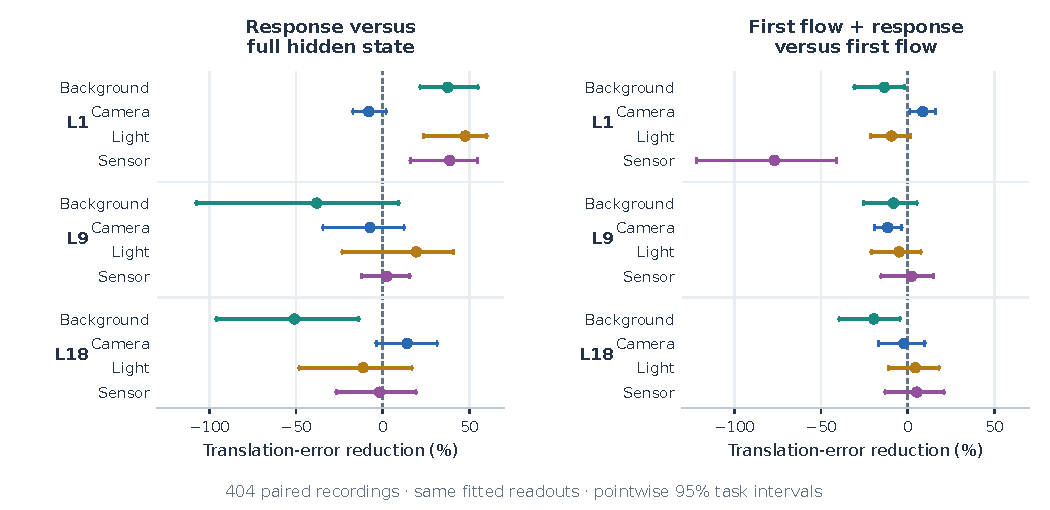
\includegraphics[width=\textwidth]{figures/supp_full_readout_controls.pdf}
\caption{\textbf{Shared coordinates mostly match the full hidden response and rarely add to first flow.} All 24 translation contrasts across three layers and four families, on the 404 matched LIBERO-Plus pairs and original task/family holdouts. Left: shared-direction coordinates versus the full hidden response. Right: first flow plus shared coordinates versus first flow. Error reduction is $100(1-\mathrm{MSE}_{\rm candidate}/\mathrm{MSE}_{\rm baseline})$; positive favors the candidate. Bars are pointwise 95\% task-component intervals under fixed fitted readouts.}
\label{fig:full-readout-controls}
\end{figure}
